\chapter{Grundlagen}

\section{Werkzeuge}
Im folgenden beschreibe ich die Werkzeuge, die ich für die Erstellung meiner Maturaarbeit gebraucht habe.
Jedes dieser Programme ist für allen grossen Betriebssystemen verfügbar.

\subsection{Unity 3D}

Unity 3D lernte ich bereits im Alter von 11 Jahren kennen.
Damals tat ich mich sehr schwer mit der englischen Sprache, konnte aber schon dann mit der Hilfe eines Buches und meines Vaters kleinere \glqq Spiele\grqq programmieren.
Dazu kommmt, dass Unity im Unterschied zu anderen (teils kostenpflichtigen) Programmen sehr einfach zu handhaben ist, durch diese Einfachheit aber nichts an Optionen und Möglichkeiten einbüsst. Deshalb habe ich mich für Unity als Programmierumgebung meiner Maturaarbeit entschieden. Die Umgebung ist folgendermassen aufgebaut\footfullcite{unity3doverview}:

\begin{figure}[H]
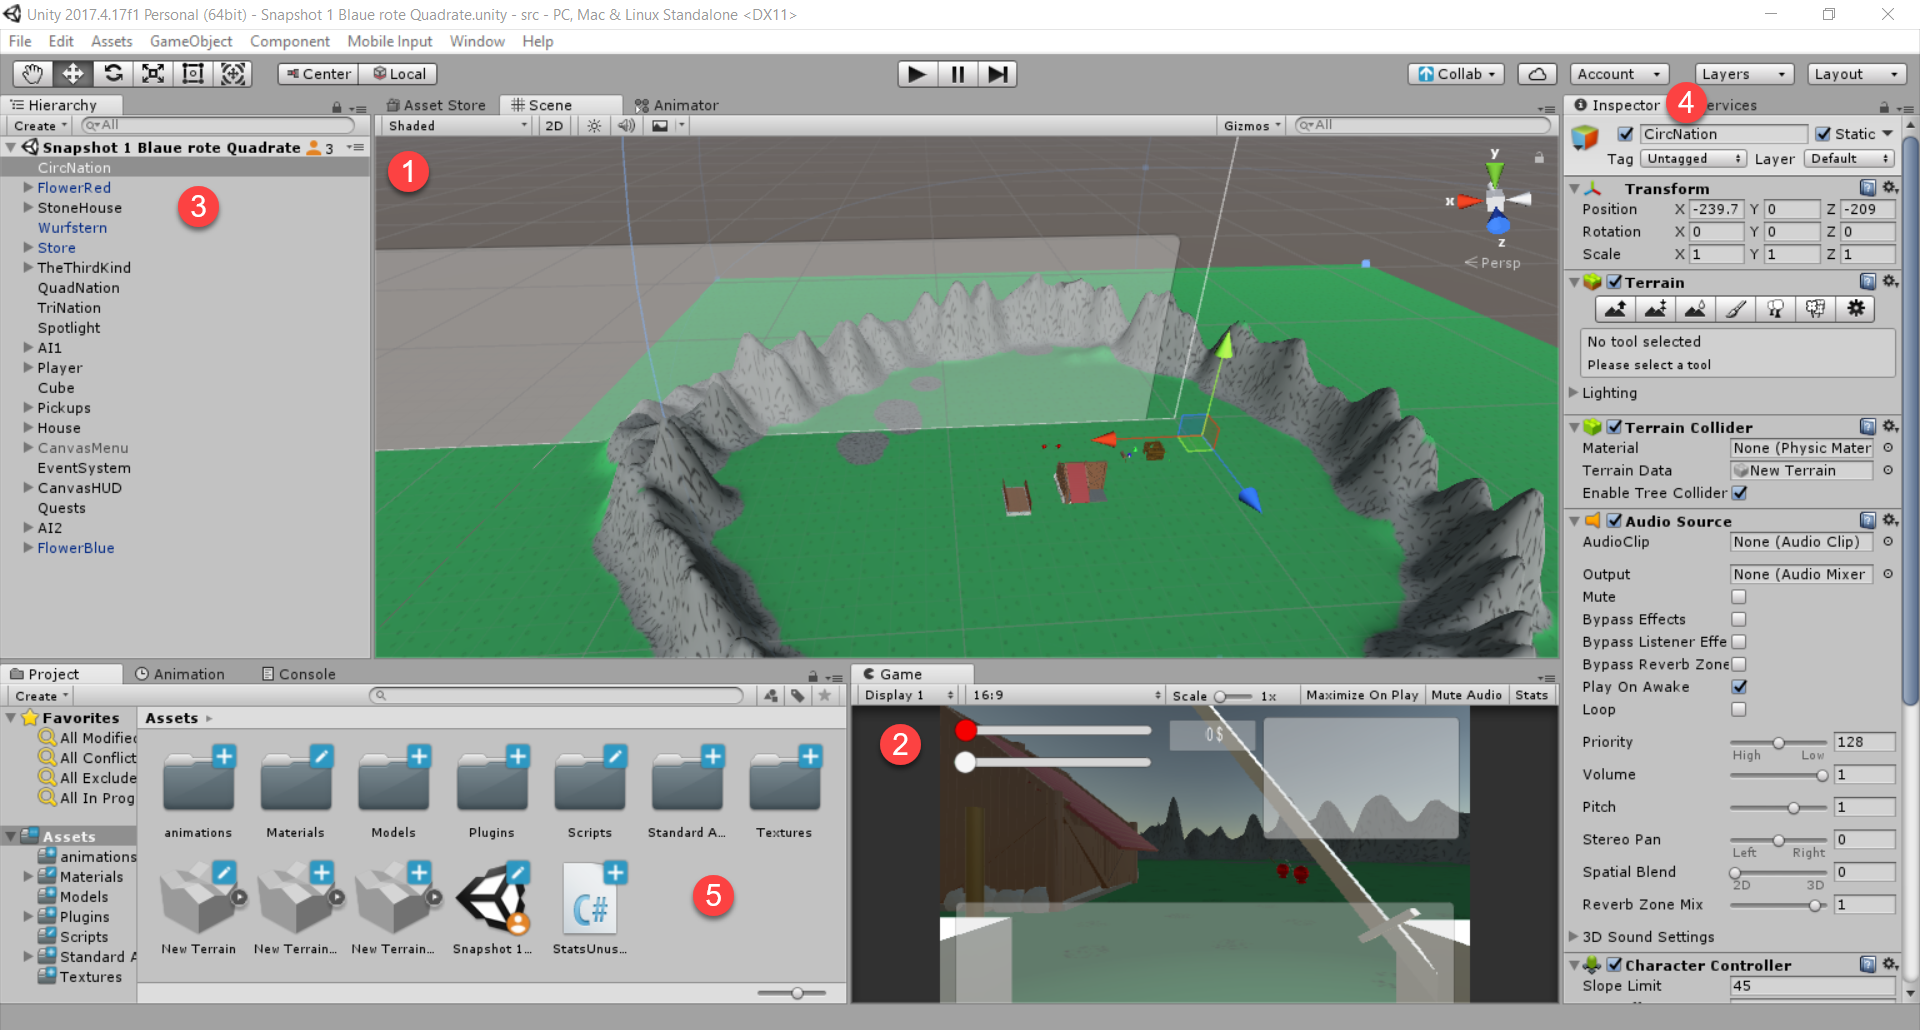
\includegraphics[scale=0.4]{screenshots/unityide.png}
\caption{Unity Benutzeroberfläche}
\end{figure}

\paragraph{Scene View (1)}
Dieses Fenster ermöglicht das Interaktive bearbeiten von Szenen und Welten.
Man kann sich in der Spielwelt überall hin und durch alle Objekte bewegen. Um Objekte zu editieren kann man sie mit X,Y und Z Achsen positionieren,
skalieren und drehen.

\paragraph{Game View (2)}
Dieses Fenster zeigt eine Vorschau des Spiels.
Sobald \textit{Play} gedrückt wird, kann man darin das Spiel spielen.
Um Veränderungen auszutesten, kann man während des Spiels pausieren, Veränderungen vornehmen und das Spiel mit diesen Veränderungen fortsetzen. Sobald der Spielvorgang durch ein zweites betätigen des \textit{Play} Buttons gestoppt wird, werden die Veränderungen wieder rückgängig gemacht.

\paragraph{Hierarchy (3)}
Dieses Fenster zeigt alle in der aktuell geöffneten Szene existierenden Objekte und deren Hierarchiestruktur.

\paragraph{Inspector (4)}
Dieses Fenster zeigt alle öffentlichen Parameter und Komponenten des aktuell ausgewählten Objekts (GameObject) an.

\paragraph{Project Browser (5)}
Dieses Fenster dient der visualisierten Navigation durch die Projektdateien \textbf{(Assets)}.
Alternativ wird in diesem Bereich die Konsole angezeigt, ein Fenster mit allen Outputs, Warnungen und Fehlermeldungen.

\paragraph{Game-Engine}
Unity liefert nicht nur die Programmierumgebung sondern auch eine selbständige Game-Engine\footfullcite{unity3dglossary}, ein spezielles Programm, welches die grundlegende Funktionalität für den selbständigen Ablauf und die Steuerung des Spieles zur Verfügung stellt, ohne dass es dafürt die Programmierumgebung braucht.


\subsection{Blender}
Blender\footfullcite{blender} ist eine frei verfügbare 3D Modellierungssoftware.
3D Modelle lassen sich damit viel besser und genauer bearbeiten als mit dem Standard Unity Editor. 
Zum Beispiel wäre das Erstellen einer komplexen Blüte in Unity ohne sehr grossen Zeitaufwand nicht möglich gewesen.

\begin{figure}[H]
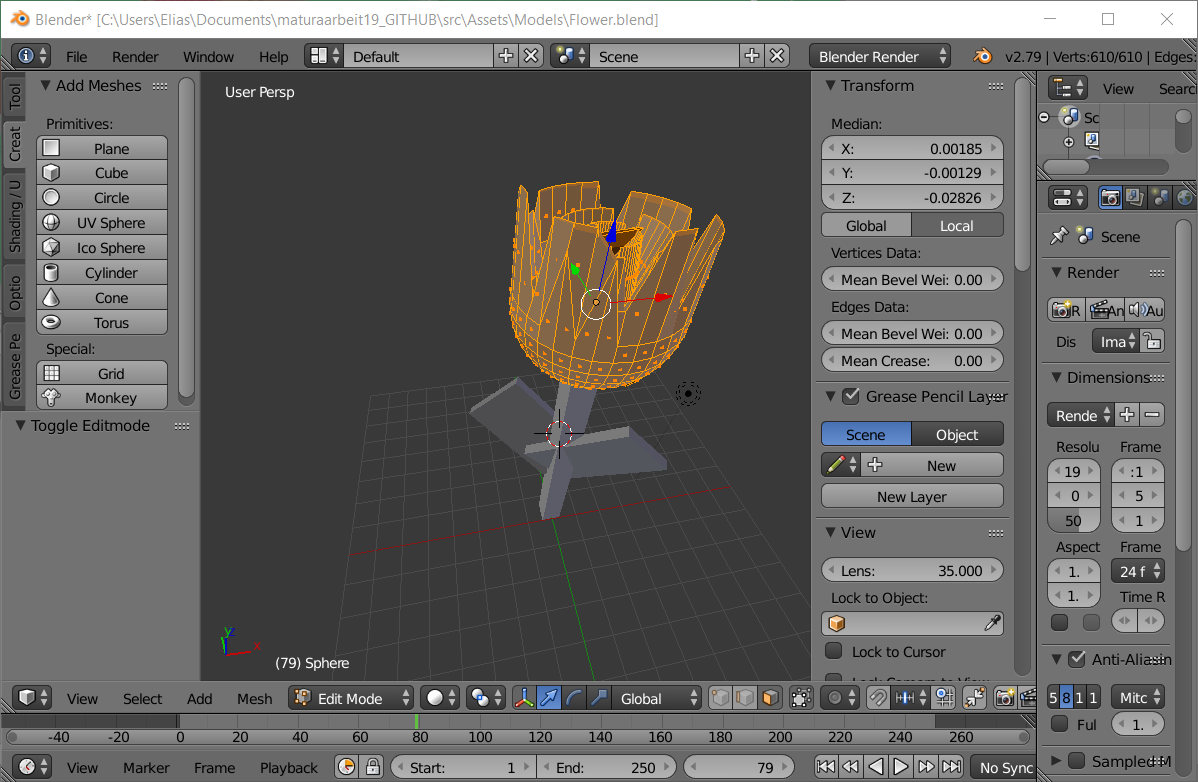
\includegraphics[scale=0.66]{screenshots/blenderflower.png}
\caption{3D Modell der Blume in Blender}
\end{figure}

\subsection{LaTeX}

Gemäss Vorgabe verfasste ich den schriftlichen Teil der Arbeit in LaTeX\footfullcite{latex}, basierend auf einer Vorlage der Kantonsschule Wattwil \footfullcite{latexwattwil}.
Als Editor verwendete ich Texmaker\footfullcite{texmaker}.

\subsection{MonoDevelop}

Scripts wurden in \textbf{MonoDevelop}\footfullcite{monodevelop} entwickelt.
Diese Umgebung verfügt über einen hochwertigen Debugger, welcher die Fehlersuche zur Laufzeit stark erleichtert.

\begin{figure}[H]
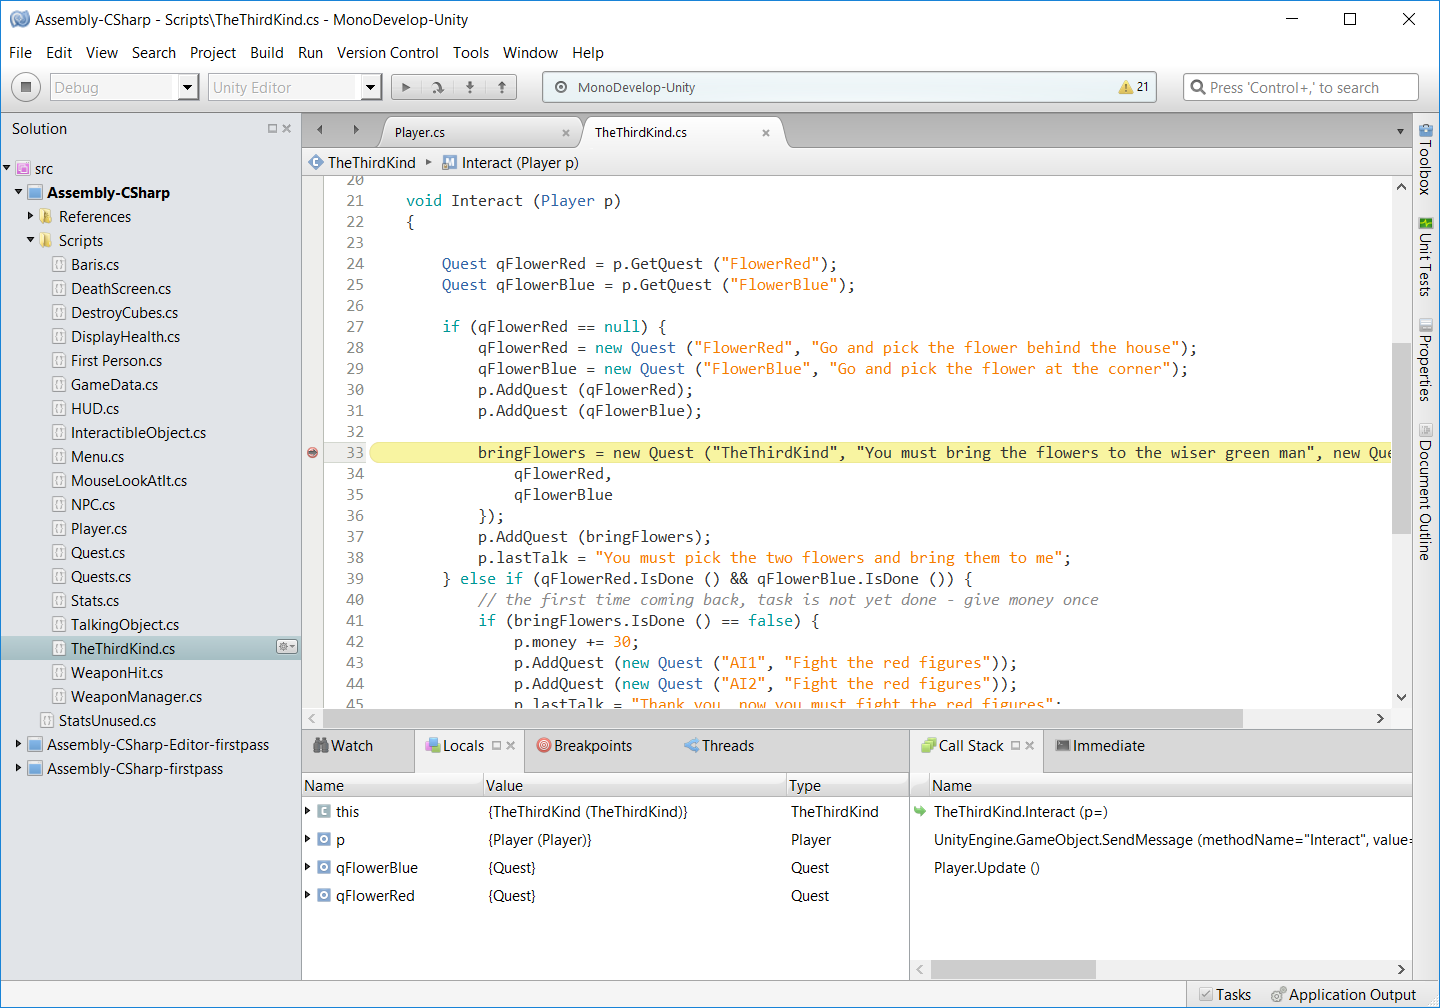
\includegraphics[scale=0.5]{screenshots/monodevelop.png}
\caption{Breakpoint im MonoDevelop Debugger mit Anzeige der Variablen}
\end{figure}

\subsection{Git}

Für die Versionsverwaltung verwendete ich das weitverbreitete Programm Git\footfullcite{git}.
Als Oberfläche kam Sourcetree\footfullcite{sourcetree} zum Einsatz.
Dafür erstellte ich mir einen Studentzugang auf Github\footfullcite{github}.
Damit wurde die Kommunikation und das schnelle Austauschen mit meiner Betreuungsperson einfacher, da man sich nicht mehr für alles treffen musste.

\subsection{astah UML}

UML Diagramme zeichnete ich mit der gratis Studentenversion von astah UML\footfullcite{astahuml}.

\section{Programmiersprache und Framework}

\subsection{C\#}
C\# ist eine objektorientierte Programmiersprache die von Microsoft entwickelt wurde\footfullcite{csharp}.
Unity kann sowohl mit C\# als auch Javascript programmiert werden.
Letzteres kannte ich schon, also habe ich die neue Sprache gewählt, um mein Basiswissen der Informatik zu vergrössern.

\subsection{Unity Framework}
Die Funktionalitäten (Klassen, Skripts etc.) bauen auf dem von Unity für nicht kommerzielle Zwecke gratis zur Verfügung gestellten Framework auf.
Ein Framework ist eine Sammlung von vorgefertigten Klassen, deren Verwendung enorm viel Zeit einspart, da sie meistens einwandfrei funktionieren und somit insgesamt weniger Zeit für die Fehlersuche aufgewendet werden muss. Gleichzeitig dient es als Grundlage für die eigenen Erweiterungen.

\footfullcite{unity3dscriptreference}.
Hier sind die zwei meist benutzten Basisklassen aufgeführt.

\subsubsection{Wichtigste Basisklassen}

\begin{figure}[H]
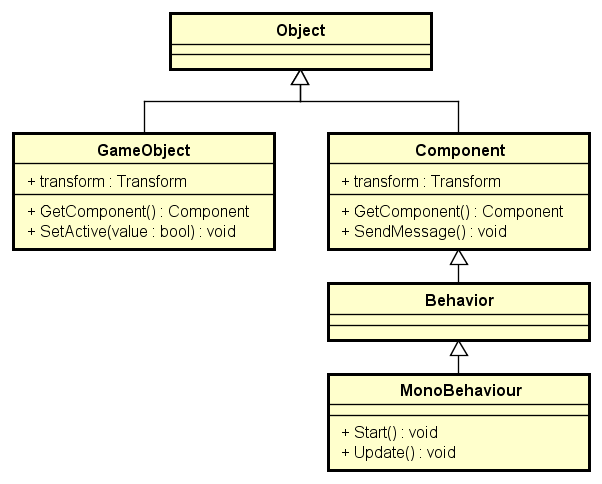
\includegraphics[scale=0.5]{diagramme/unitybaseclasses.png}
\caption{Basisklassen in Unity}
\end{figure}

\paragraph{GameObject}\footfullcite{unity3dgameobject}
GameObject ist die Basisklasse für alle Objekte, die auf der Benutzeroberfläche erstellt werden.
Die wichtigste Eigenschaft eines GameObjects ist \lstinline{transform}.
Dieses beinhaltet die Position,Drehung und Skalierung im Raum.
\lstinline{GetComponent<Komponentenklasse>} ist die meist benutzte Methode. 
Sie liefert die Komponente z.B. das Kollisionsobjekt oder Skripts des GameObjects. 
\lstinline{SetActive} aktiviert oder deaktiviert das Objekt
Ein inaktives GameObjekt wird unsichtbar und erhält keine Aufrufe mehr.

\paragraph{MonoBehaviour}\footfullcite{unity3dmonobehaviour}

MonoBehaviour ist die Basisklasse wenn ein GameObject mit einem Skript erweitert wird.
Die zwei geerbten Methoden die standardmässig überschrieben werden sind:
\lstinline{Start()} wird zu Laufzeitbeginn ein mal aufgerufen.
Es wird benutzt um Initialisierungen durchzuführen.

\lstinline{Update()} wird jedes Mal aufgerufen bevor ein neues Bild des Spiels berechnet wird. In abgeleiteten Klassen werden in dieser Methode deshalb Elemente wie Bewegungen fortlaufend aktualisiert.
\lstinline{SendMessage} übermittelt einen Aufruf an alle Komponenten des Objekts.

\subsubsection{Input-Manager}

Der Inputmanager\footfullcite{unity3dinputmanager} dient der virtuellen Steuerung des Spielers. Er kann z.B. nach Achsen (vorwärts, seitwärts) abgefragt werden und deren Intensität mitliefern.
Die Zuordnung von Tasten zu Achsen kann angepasst werden:

\begin{figure}[H]
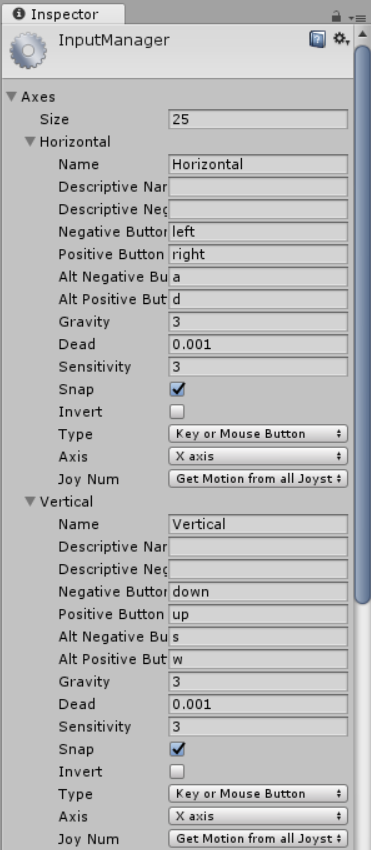
\includegraphics[scale=0.67]{screenshots/inputaxis.png}
\caption{Der Inputmanager mit horizontaler und vertikaler Achse zugeordnet an die Tasten a-d/s-w}
\end{figure}

Die Abfrage im Code sieht folgendermassen aus:

\begin{lstlisting}[caption={Abfrage der X- und Z-Achsen im Code}]
private void Update ()
{
	(...)
	// x und z Koordinaten Bewegung
	float x = Input.GetAxis ("Horizontal") * Time.deltaTime * speed;
	float z = Input.GetAxis ("Vertical") * Time.deltaTime * speed;
	(...)
}      
\end{lstlisting}

\subsection{Physik}

\subsubsection{Rigidbody}
Jedes GameObject, auf welches sich physikalische Kräfte wie Gravitation auswirken, besitzt einen Rigidbody\footfullcite{unity3drigidbodyoverview}.
\begin{figure}[H]
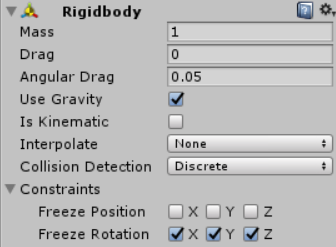
\includegraphics[scale=0.8]{screenshots/rigidbody.png}
\caption{Rigidbodykomponente}
\end{figure}
Hier wird die Masse des Players auf 1 festgelegt. Dies wird z.B. beim Berechnen des Springens verwendet.

\subsubsection{Kollisionen}
\label{subsubsec:collider}
Die Kollisionserkennung ist einer der wichtigsten Bestandteile eines Spiels. Sie wird nicht nur für die Geltendmachung eines Treffers verwendet, sondern sie entscheidet auch, wann z.B. ein Element im Sichtfeld eines Spielers ist oder nicht.
Die Hauptkomponente für das Feststellen einer Kollision ist der Collider.
Dessen Umrisse werden in der IDE definiert.
\begin{figure}[H]
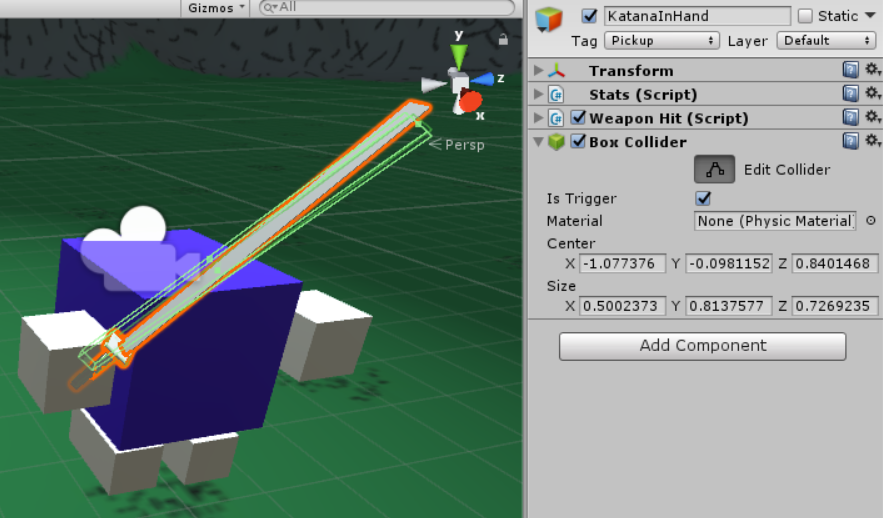
\includegraphics[scale=0.8]{screenshots/katanacollider.png}
\caption{Kollisionskomponente des Katanas}
\end{figure}
Hier sieht man den Collider in Grün. Man sieht dass er nicht die ganze Waffe abdeckt, da nur die Klinge als Trefferzone gelten soll.

Um diese Kollision einem Skript zu übermitteln gibt es zwei Methodengruppen.
\paragraph{\lstinline{OnCollisionEnter/Stay/Exit}} wird ausgelöst, sobald ein Physikalischer Treffer zwischen zwei Körpern festgestellt wird.
\paragraph{\lstinline{OnTriggerEnter/Stay/Exit}} wird ausgelöst, wenn ein designierter Collider getroffen wird. Dieser muss hierbei nicht zwischen zwei Körpern stattfinden, sondern z.B. bei Eintreten in ein Sichtfeld (\cref{subsubsec:npc}).






